
\section{FSL FIX}

The following section will describe the implementation of the automated de-noising system FIX, which introduces a faster and more standardized approach to ICA-based noise cleanup \cite{Salimi-Khorshidi2014}. The FIX method is a more extensive approach, which adds another layer of analyses to the standard preprocessing. This means that before initiating FIX the data needed to undergo the exact same steps as in the standard preprocessing presented in \secref{sec:std}. Following the standard preprocessing, the functional scan underwent an ICA to separate the sources in the acquired signal and ideally splitting signal of interest and noise. Afterwards an analysis of optimal number components in which the signal should be split was performed, as the initial results from the default setting were assessed not to sufficiently separate the signal sources. The FIX method uses a classifier to separate noise components from signal components. Hence a classifier made and trained in doing this separation. In \figref{fig:meth:fix} a flowchart showing the steps for both the training data set and the test data set in the FIX pipeline is illustrated. 


\begin{figure}[H]                 
	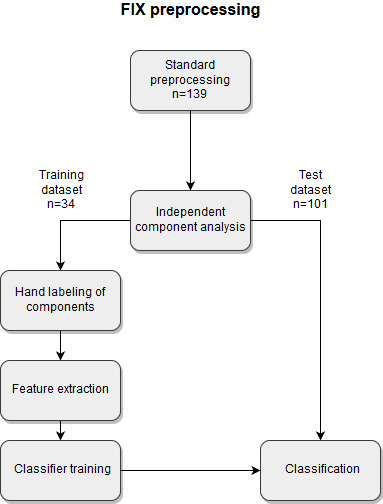
\includegraphics[width=.6\textwidth]{figures/bMethods/FIX_flow} 
	\caption{Flowchart illustrating the two datasets and the corresponding steps that was applied to each dataset in the FIX pipeline.}
	\label{fig:meth:fix} 
\end{figure}

%
%
%\subsection{Calculation of Independent Components}
%
% For a single session ICA the MELODIC FSL program utilizes the FastICA algorithm to obtain independent components. This section seeks to lay out how the FastICA algorithm works and which mathematical techniques that are exploited. \\
% As stated in \secref{sec:ICA}, from the central limit theorem we get that observed mixed signals tend to have a more Gaussian distribution than the individual source signals, since the observed signal is a summation of the source signals. As a result of this, an approach is to find a linear transformation that leaves the source signals as non-Gaussian as possible. This principle is what the FastICA algorithm is build up around. \\
% Firstly the vector \textbf{b} is introduced, which is a row vector in the mixing matrix \textbf{A}, and is used in a linear combination:
% 
% \begin{equation}
% y = \mathbf{b^T}\mathbf{x}
% \end{equation}
% 
% By substituting $\mathbf{x} = \mathbf{A}\mathbf{s}$ in the previous equation:
% 
% \begin{equation}
% y = \mathbf{b^T}\mathbf{A}\mathbf{s} = \mathbf{q^T}\mathbf{s}
% \end{equation}
% 
% Where $\mathbf{q^T} = \mathbf{b^T}\mathbf{A}$. From this it can be deduced that \textit{y} is an IC, when only one of the entries of \textbf{q} is non-zero and the rest is zero. This means that there is no addition of any random processes and the component will be as non-Gaussian as possible. An IC can then be obtained by calculating a value of \textbf{b} that maximizes the non-Gaussianity of the distribution of $\mathbf{b^T}\mathbf{x}$ as $\mathbf{b^T}\mathbf{x} = \mathbf{q^T}\mathbf{s}$. This gives an optimization problem with convergence at local maxima. As there exist a local maximum of the non-Gaussianity for both \textit{s} and ${s_i}$, the optimization landscape in a n-dimensional signal gives a total of \textit{2n} local maxima.
% To be able to optimize according to non-Gaussianity, a quantitative measure of such is needed. This can be provided by the fourth order cumulant, kurtosis, which is zero when \textit{y} is Gaussian distributed and non-zero when \textit{y} is non-Gaussian distributed (negative when sub-Gaussian and positive when super-Gaussian). Given this property and the central limit theorem, the linear combination $\mathbf{b^T}\mathbf{x}$ that yields an IC can be found at the local maxima of the absolute value of the kurtosis of \textit{y}. The kurtosis of \textit{y} is given by:
% 		
%\begin{equation}
%kurt(y) = E{y^4} - 3E{y^2}^2
%\end{equation}
% 		
%As the whitening of the data results in unit-variance, \textit{kurt(y)} can be modified to:
%		
%\begin{equation}
%kurt(y) = E{y^4} - 3
%\end{equation}
% 		
%To simplify the theoretical analysis furthermore the linear properties of kurtosis for sums of variables can be utilized. For two random variables, \textit{$x_1$} and \textit{$x_2$}, it holds that:
%
%\begin{equation}
%\begin{split}
%kurt(x_1 + x_2) &= kurt(x_1) + kurt(x_2) \\
%kurt(\alpha x_1) &= \alpha^4 kurt(x_1)
%\end{split}
%\end{equation} 			
%For the multiplicative scalar textit{$\alpha$} the kurtosis is non-linear, and the optimization problem can thus be written as:
% 			
%\begin{equation}
%kurt(y) = \sum_{i} q_{i}^{4}kurt(s_i)
%\end{equation}
% 			
%Due to the whitening of the data, where \textit{y} has unit-variance, a constraint is put on the vector \textbf{q}. Since $E{y^2} = \sum_{i}^{n} q_{i}^{4}$ the vector \textbf{q} is constrained to the unit-sphere. For the whitened data \textbf{z} a linear combination $\mathbf{w^T}\mathbf{z}$ that maximizes non-Gaussianity is sought for. From the fact that $\mathbf{q} = \mathbf{V}\mathbf{A})^{T}\mathbf{w}$, the following is given:
% 			
%\begin{equation}
%\parallel \mathbf{q} \parallel^{2}= (\mathbf{w}^{T}\mathbf{V}\mathbf{A})(\mathbf{A}^{T}\mathbf{V}^{T}\mathbf{w}) = \parallel \mathbf{w} \parallel^{2}
%\end{equation}
% 			
%This expresses that constraining the vector \textbf{q} to lie on the unit sphere equally constraints \textbf{w} to the unit sphere. The objective is now to find a value of \textbf{w} that maximizes the absolute value of the kurtosis of $\mathbf{w^T}\mathbf{z}$. Whitening further allows the linear combination $\mathbf{w^T}\mathbf{z}$ to be understood as projections on the line in a 1-D subspace spanned by \textbf{w}. What is sought for is the direction of \textbf{w} where the absolute value is maximized, which then makes out an IC. \\
%To solve this optimization problem a commonly used technique is the gradient algorithm to reach convergence at local maxima, thus calculating the direction where the absolute value of the kurtosis of $\mathbf{w^T}\mathbf{z}$ is growing most strongly. The can be computed as the following:
% 			
%\begin{equation}
%\frac{\delta|kurt(\mathbf{w^T}\mathbf{x})|}{\mathbf\delta\varTheta{w}} = 4 ~ sign ~ (kurt(\mathbf{w^T}\mathbf{z})[E{\mathbf{z}(\mathbf{w^T}\mathbf{z})^{3}} - 3\mathbf{w}\parallel\mathbf{z}\parallel ^{2}]
%\end{equation}
% 				
%However, there is in practice disadvantages associated with using the gradient algorithm, e.g. slow convergence rate and is dependent on a proper choice of learning rate. The fixed point algorithms is suggested as a faster algorithm alternative. At the stable point of the gradient algorithm, the gradient is pointing the direction of \textbf{w}. It is only in this case that \textbf{w} will not change direction when adding the gradient. This notion about the gradient of the absolute value of the kurtosis can be used to form a fast fixed point algorithm, or the FastICA algorithm:
% 				
%\begin{enumerate}
%\item $\mathbf{w}  \leftarrow  E\{{\mathbf{z}(\mathbf{w^{T}\mathbf{z})^3}}\} - 3\mathbf{w}$
%\item $\mathbf{w}  \leftarrow \mathbf{w} / \parallel \mathbf{w} \parallel$
%\end{enumerate}
% 									
% 					
%The right hand side is firstly computed and assigned to \textbf{w}, which afterwards is normalized to follow the constraint of $\parallel \mathbf{w} \parallel ^2 = 1$. By iterating over this convergence is reached at an ultimate \textbf{w}, where $\mathbf{w^{T}\mathbf{z}}$ is an IC. In order to obtain several IC’s the process is repeated, with the constraint that \textbf{w} must be orthogonal to all previously computed \textbf{w}. 
% 						